\chapter{Scraper Design and Implementation}\label{C:us}

In this section I discuss the design and implementation of the web scraping components of the project. I highlight important decisions made during the course of the project, as well as steps taken to implement the system based on requirements detailed in chapter four.

\section{A Prototyping Approach}

The overall design of my scrapers was largely developed through a prototyping approach early in the project. I performed research and web-scraping frameworks and technologies to decide which would best suit the requirements defined in chapter 4. The prototyping strategy also allowed me to investigate the feasiblity of scraping from different sites.

By developing prototypes for Facebook and Twitter early in the project I was better able to 

\section{Architecture}

Through the development of these basic prototypes, construction of more formal architectures was possible. I consider two architectures, when designing the web-scraper components. A database-storage approach was considered, and the more straightforward text/XML storage architecture was also considered and ultimately selected. 

\subsection{Database Storage Architecture}

A possible approach to meeting the goals of the project was to store fetched data in a relational database. In this design, the scrapers would gather data over an extended period of time, writing retrieved data into a database. Analysis components would then fetch data from the database storage as necessary, saving results in seperate tables within the same database.

This approach provides benefits in terms of long-term extensibility of the project. All of the advantages that come with database storage would have been present in this solution - 

The drawbacks to this approach are to do with the deemed over-engineered nature of the solution. Given that data retrieved is HTML, there was a large impedance mistmatch between data retrieved and the relational database format. This would then need to be converted back into object format for analysis. 


Advantages - relational model, persistance, backups. Simplicty of fetching exact data.

Disadvantages - extra complexity deemed unnecessary. Worse integration with GRAft. 

\begin{figure}[h!]
 \centering
 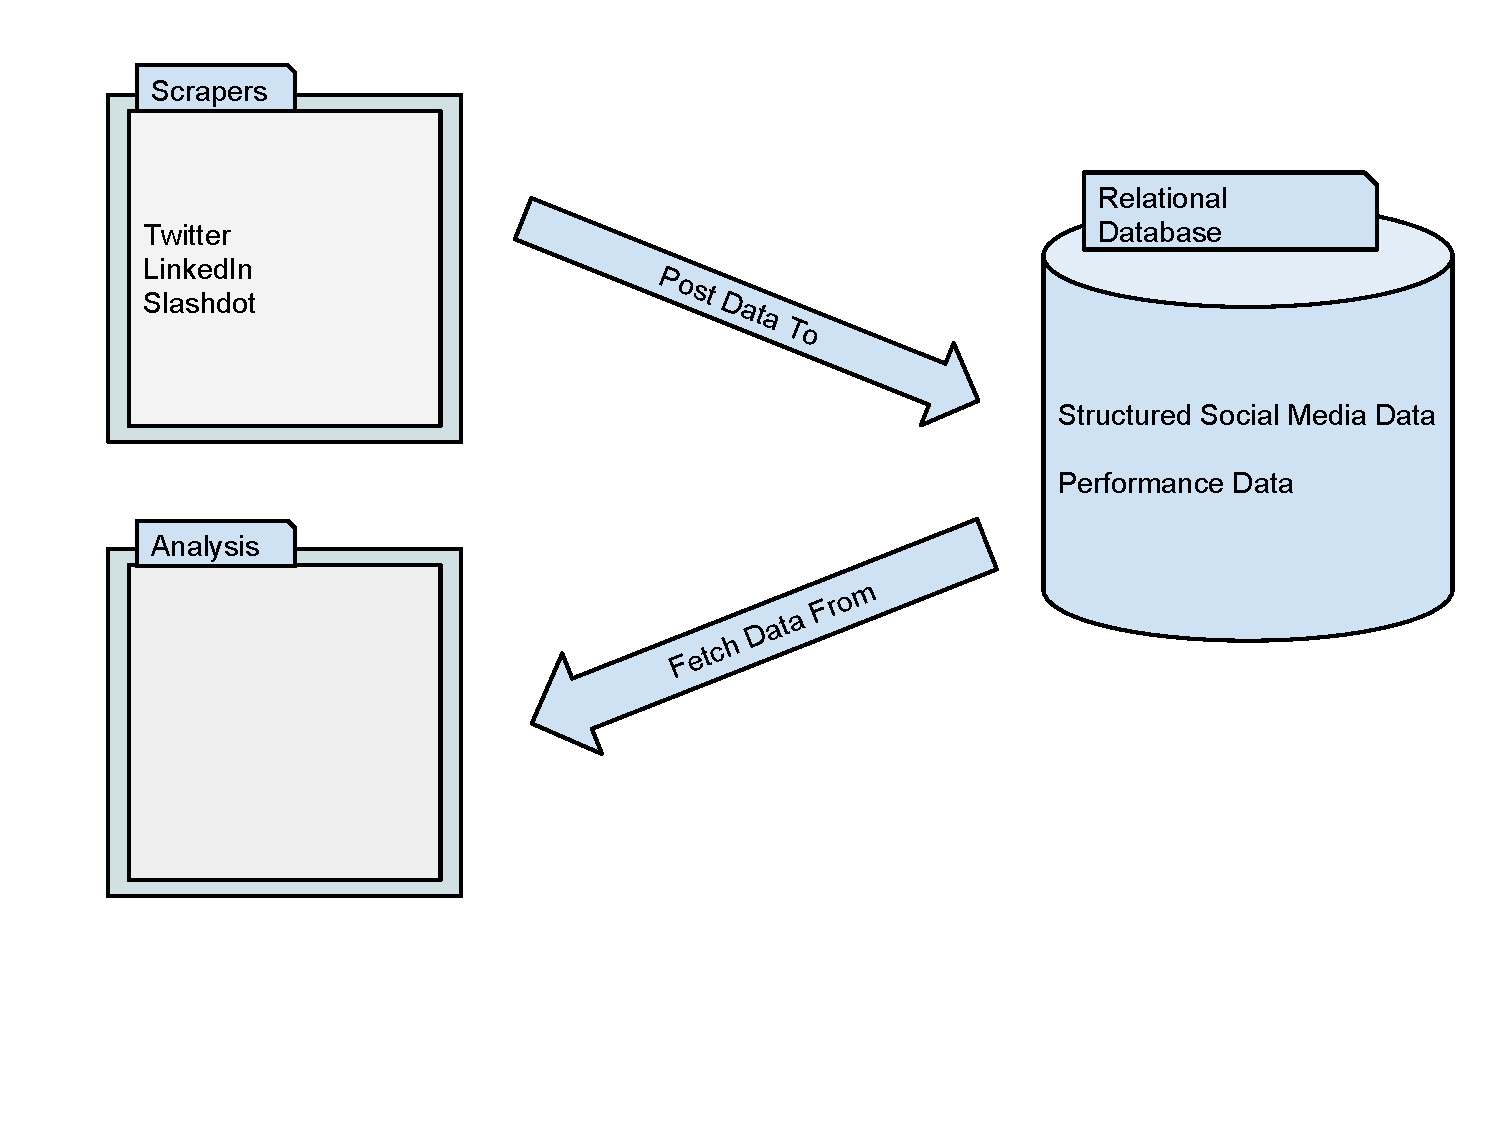
\includegraphics[width=0.5\textwidth]{Images/Database_Architecture.pdf}
 \caption{Proposed Architecture for Database Storage Solution}
\end{figure}

\subsection{XML Storage Architecture}

Advantages - simplicty of scripting. Simplicty of integration with GRAft. Simplicity of changing structures. 

\begin{figure}[h!]
\centering
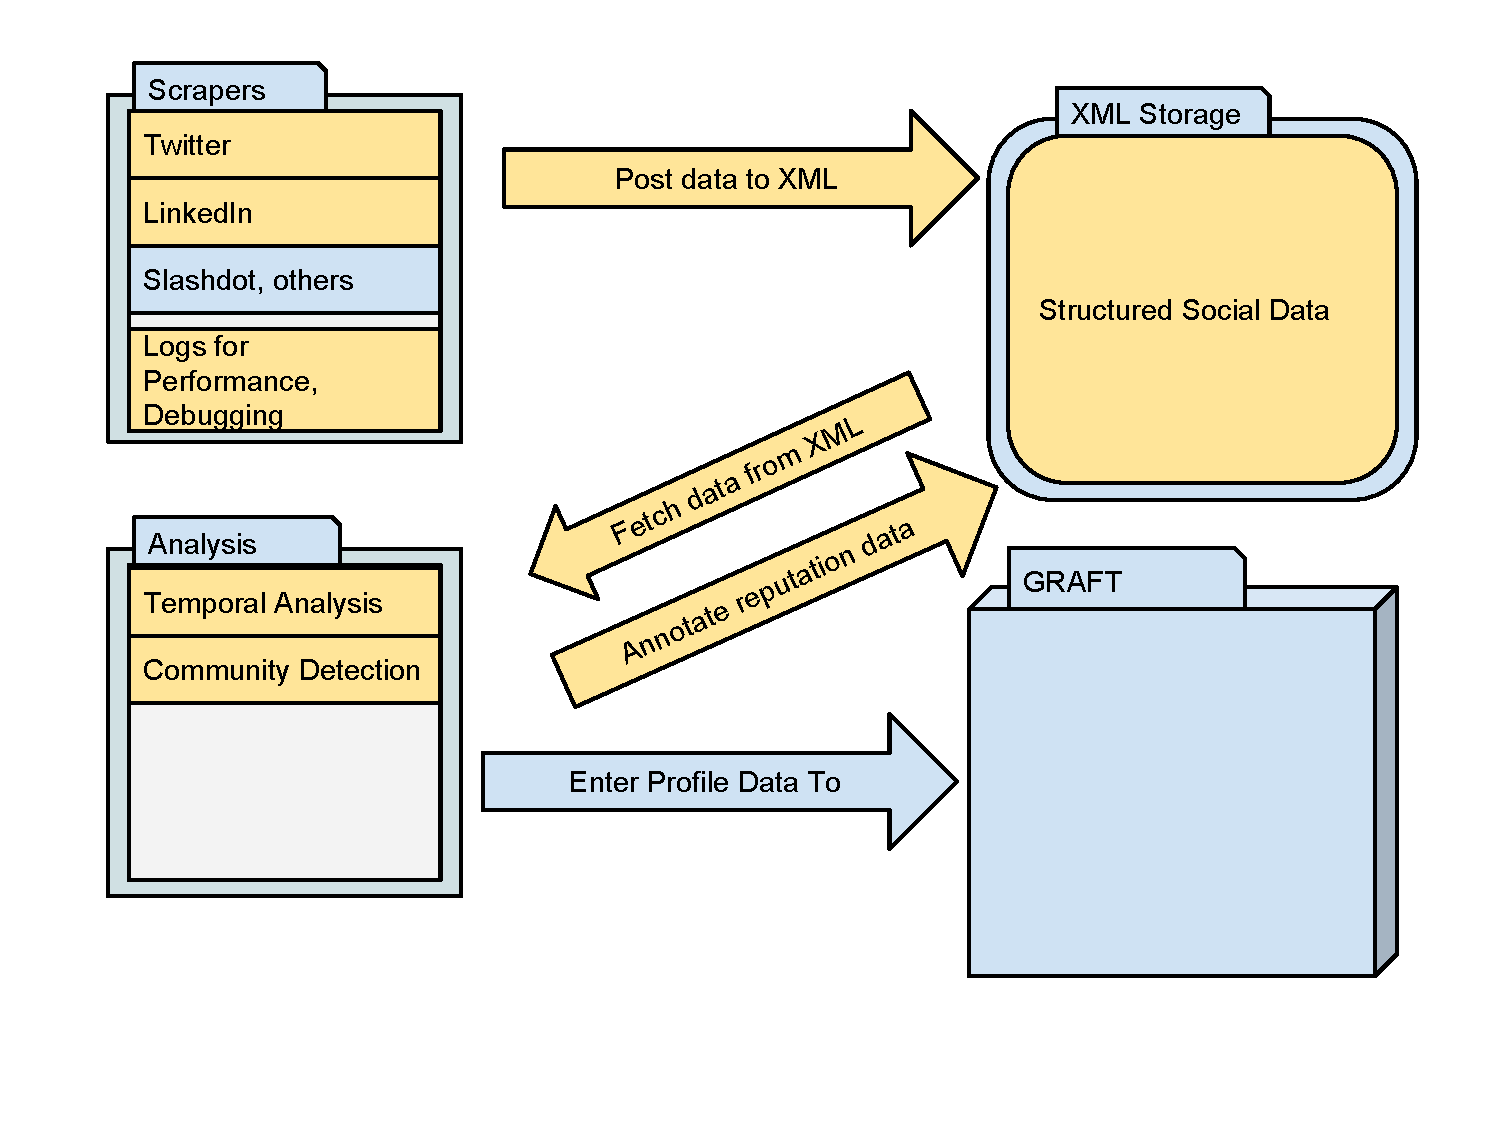
\includegraphics[width=0.5\textwidth]{Images/XML_Storage_Architecture.pdf}
\caption{Proposed Architecture for XML Storage Solution}
\end{figure}

\section{Technology}

My scrapers were written entirely in Ruby. Developing screen scrapers is largely independant upon language choice; however Ruby was selected due to its large number of libraries suitable for scraping, and straightforward scripting nature. Ruby also has a significant OpenSource culture in comparison to many other languages.This was considered important early in the project when looking at developing a model for future maintenance of the scrapers, especially when considering the discarded requirement of aggregating data for GRAft. 

Alternatives to Ruby were considered; Java, which does not have the same open source following as Ruby, as well as a larger degree of lower-level network coding for web-scraping software; and PHP, which was rejected due to personal time constraints restricting personal capabilities of learning the language to a competent level during the project. PHP would have given the advantage of being more consistent with past works, however \cite{GRAft}, as well as being the same language as my policies are described in. 

The frameworks upon which my scrapers are built included:

\begin{itemize}
 \item Nokogiri: a widely used HTML and XML parsing library, allowing for straightforward interpretation of raw HTML documents.
 \item Mechanize: a library simulating browser interaction on web-pages, without requiring a real browser.
 \item Rest-Client: Ruby's most popular HTTP client.
\end{itemize}

\begin{figure}[h!]
\centering
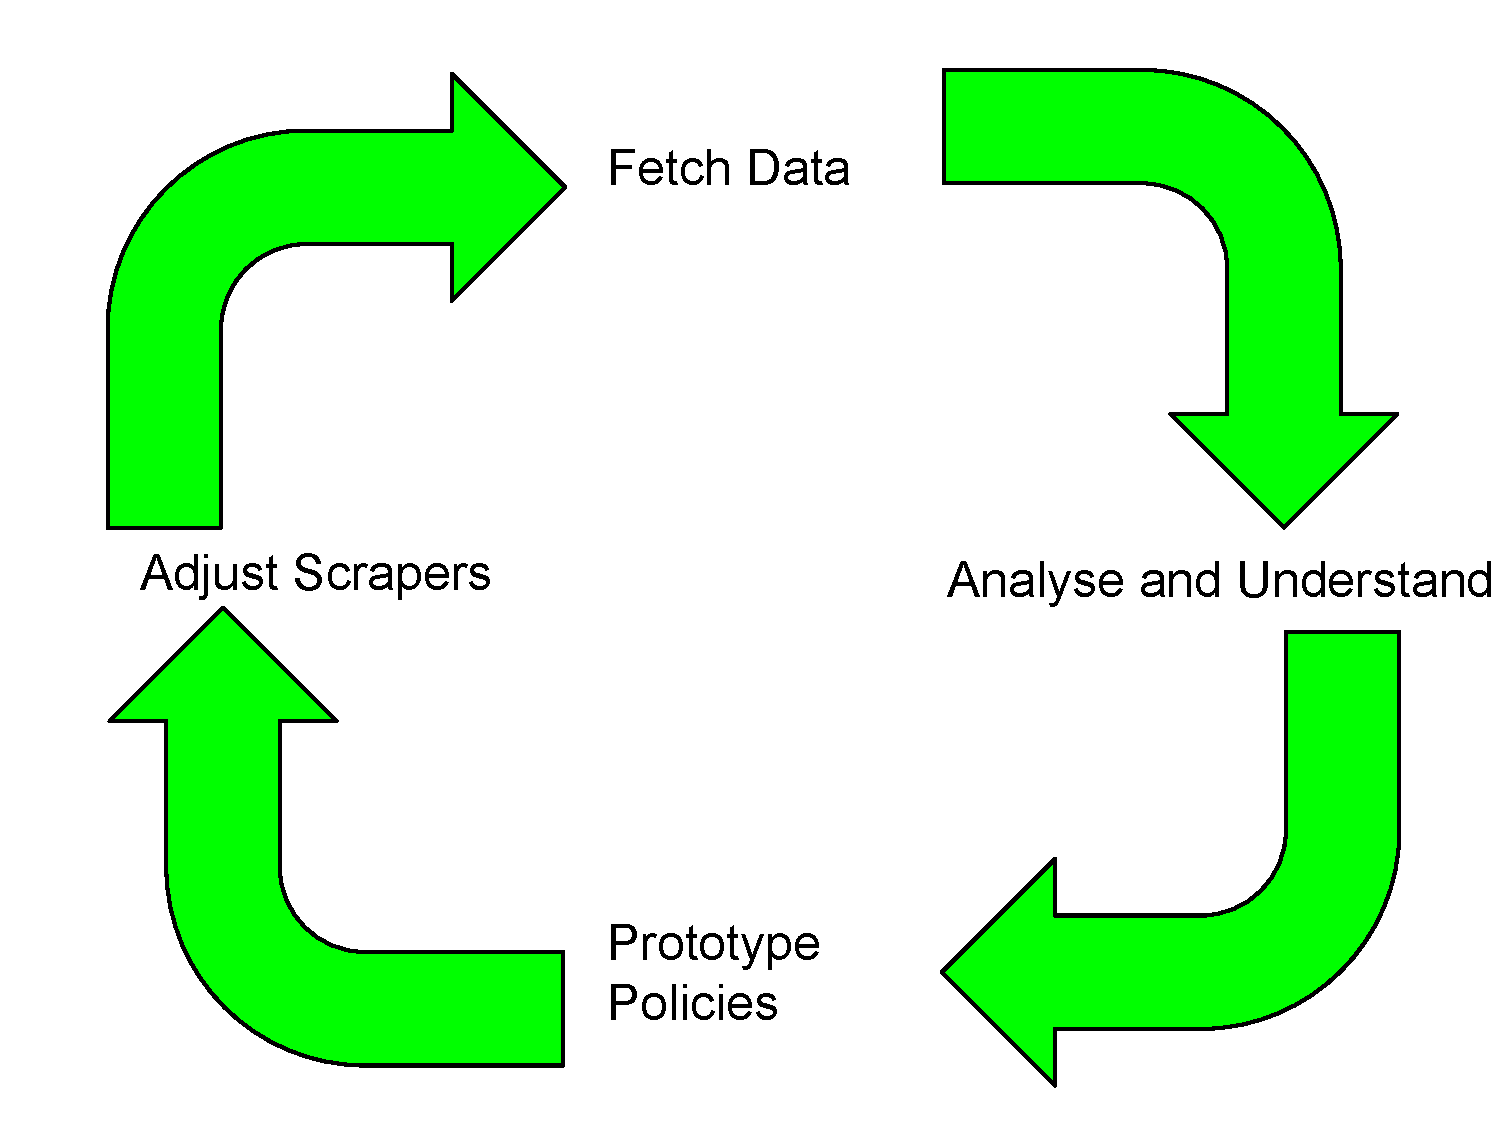
\includegraphics[width=0.7\textwidth]{Images/Implementation_Lifecycle.pdf}
\caption{Scraper Development Feedback Loop}
\end{figure}



\subsection{Systems Design and Structure}

Developing the project solution consisted generally of a cyclic, iterative prototyping approach as detailed in figure 5.1. This generally consisted of four phases; Implementing and adjusting scrapers, fetching data, analysing the data, and prototyping policy concepts as a result of this analysis. 

Various frameworks were considered when implementing my standalone scraping application. Option one was to extend scrAPI, a Rubyforge project allowing for rapid development of web scrapers. The primary benefit claimed by scrAPI is that it would allow me to fetch data from HTML pages using CSS selectors. It also hid processes such as the actual fetching of pages, and sending of HTTP requests. 


Browser automation options were considered as an alternative architecture. Libraries such as Watir allow users to simulate user interaction with web pages, by driving an actual browser instance. Watir - browser automated option. More for automated tests. Performance would be significantly worse than nokogiri, as pages are loaded through the browser. Also personal experience from building such applications shows that implementation of such a solution would be very time consuming. Advantages of this would be low detection rates.  

%This is where I should incorporate the discussion about framework selection.

\subsection{Code instrumentation}

The code was instrumented using a Ruby logger system written for the application. Given complexities and difficulties debugging errors on web-scraping applications, logging had to be performed to a very fine level of granularity. Any action changing system state such as fetching a page triggers the logging mechanism. The logger would then take note of the timestamp and write to the appropriate file the nature of the action. For example, if the scraper sent an HTTP request to retrieve a given URL, it would record the timestamp and URL requested. 

The logger would write to the appropriate log file based on the nature of the supplied action. Because these scrapers were running over long periods of time, using traditional IDE debugging tools was not effective at detecting errors. As a result, I used multiple debugging files with different purposes in an attempt to catch these errors. The debug.log captured all interaction information at a basic level. Error.log captures error information that is non-fatal to scraping an individual's profile, e.g. on Twitter. Commonly these errors were due to application logic flaws, such as performing operations on null entities. As a result the error.log assisted greatly in identifying these edge cases. Finally the failure.log was used to record fatal exceptions that would prevent me from scraping a profile. Occurences such as 404, 500 or 503 responses from servers are examples that would result in a record being written to the failure log. The failure log would write system state at the time of failure to a high level 
of detail, sometimes even writing the entire HTML document before the failure to disk. This again assisted with debugging, when reviewing how a particular run had gone. 

To limit the performance overhead of writing to these logging files, a buffered approach was taken in order to achieve the least impact. %lol

\section{Dataset} %Or should this be placed in evaluation.

\subsection{Extend scrAPI}

scrAPI is a Rubyforge project, allowing for fast implementation of web scrapers. The benefit of scrAPI is that it would allow me to fetch data from HTML pages using CSS selectors. It also hid processes such as the actual fetching of pages, and sending of HTTP requests. Ultimately scrAPI was a more high-level approach to scraping content.

Extending scrAPI was ultimately discarded however, due to its heavy reliance on CSS files remaining constant. Any change to stylesheet files would likely have broken my scrapers. Arguably these stylesheets are less likely to change than layout manipulations (e.g. consider xpath on HTML as an alternative); however on sites such as Twitter and Facebook large design teams frequently make changes to these files. Given that a key requirement of the project was to make scrapers resistant to user-interface change, this resulted in scrAPI being deemed unfit for purpose. 

\subsection{Extend A Browser-Automation Model}

Browser automation options were considered as an alternative architecture. Libraries such as Watir allow users to 

Watir - browser automated option. More for automated tests. Performance would be significantly worse than nokogiri, as pages are loaded through the browser. Also personal experience from building such applications shows that implementation of such a solution would be very time consuming. Advantages of this would be low detection rates. 

\section{Social Media Selection}

In order to scrape useful information, I needed to look at the various social media sites in the context of gathering reputation data, and seeing what could be selected. 

\subsection{Standalone Crawling Application}

A standalone crawling application architecture was considered, and ultimately chosen as the most suitable strategy. 

\section{Product Implementation}

\subsection{Technology Choice}

%THIS is where I talk about the various technologies that were considered. Browser automation and the like. 

%State why I chose this architecture, and how I built the application.

%Discuss some of the difficulties I faced, Infinite Scroll, Quantifying Reputation Data, Sites Requiring Authentication.

%Sites with large amounts of interactive and dynamic content are significantly more difficult to scrape data from.

\subsection{Twitter Scraper}

%How I went about implementing the Twitter scraper

Initial prototype

Design improvements, including multi-threading and parallel fetching of tweets. Decisions around discarding requests that fail in scraping individual tweets. 

\subsection{LinkedIn Scraper}

\subsection{Facebook Scraper}





%Define the architectures that I considered for implementing web-scraper

%Option one - stand-alone web scraping libraries

%Option two - extend existing web scraper, utilise this.